\documentclass[a4paper,oneside]{book}
\usepackage{anysize}
\usepackage{lastpage}
\usepackage{fancyhdr}
\usepackage{polyglossia}
\setdefaultlanguage[variant=uk]{english}
\usepackage{fontspec}
\usepackage{color}
\definecolor{bkg}{rgb}{0.9,0.9,0.9}
\definecolor{cmt}{rgb}{0.0,0.6,0.0}
\usepackage{fancybox}
\usepackage{listings}
\defaultfontfeatures{Ligatures=TeX}
\usepackage{graphicx}
\graphicspath{{./logo/}{.}}
\usepackage[x11names]{xcolor}
\usepackage[colorlinks=true]{hyperref}
\usepackage{framed}
\usepackage{float}
\usepackage{wrapfig}
\restylefloat{figure}
\usepackage{makeidx}
\usepackage{listings}
\lstset{
  backgroundcolor=\color{bkg},
  basicstyle=\small\ttfamily,
  breaklines=true,
  columns=fullflexible,
  numbers=left,
  numberstyle=\tiny,
  keywordstyle=\color{blue},
  commentstyle=\color{cmt},
  stepnumber=5,
  captionpos=b,
}
\lstdefinelanguage{json}{
  morecomment=[l]{//},
}
\usepackage{caption}
\usepackage{subcaption}

\marginsize{1.5cm}{1.5cm}{0.5cm}{1.7cm}
\pagestyle{plain}
\setmainfont{Reporter}
\makeindex

\begin{document}
\begin{figure}[h]
  \includegraphics[width=\textwidth]{doc_head.jpg}
\end{figure}

\parindent=0pt
\parskip=0.25cm

\begin{center}
\fontsize{20}{21}\selectfont

\textbf{GazeToMouse}:\\
Usage of the \textbf{Tobii Eye Tracker 4C}\\
from within a \textbf{ztree} program\\
\vskip 6mm
Tutorial
\vskip 6mm

\fontsize{13}{14}\selectfont
Simon Maurer - \texttt{simon.maurer@humdek.unibe.ch}\\
\today
\end{center}

\tableofcontents

\chapter{Introduction}\label{sec.intro}
This documents describes how to use the \href{https://tobiigaming.com/eye-tracker-4c/}{Tobii Eye Tracker 4C} in order to track the gaze of a subject and feed the gaze data to the mouse device.
This allows to use the eye tracker to control the mouse pointer position such that the mouse pointer is placed at the screen coordinates where the subject is gazing at.
This documentation comes with a set of tools (executable .exe files) that provide this functionality as well as some auxiliary tools that help to calibrate and test the eye tracker.

The project aims at providing a set of executables which allow to use the \href{https://tobiigaming.com/eye-tracker-4c/}{Tobii Eye Tracker 4C} in conjunction with \href{http://www.ztree.uzh.ch/en.html}{ztree} to perform economic experiments.
The following set of executables are provided:
\begin{description}
    \item[TobiiCalibrate.exe] This program is a simple wrapper for the Tobii calibration tool.
        It launches the calibration GUI where the subject is led through the calibration process.
        The calibration data is stored in the current profile of the eye tracker engine.
    \item[TobiiGuestCalibrate.exe] This program is a simple wrapper for the Tobii guest calibration tool.
        Similar to \texttt{TobiiCalibrate.exe} it launches the calibration tool, however, the calibration data is stored in a guest profile.
    \item[TobiiTest.exe] This program is a simple wrapper for the Tobii eye tracking testing tool.
        It launches a GUI where the result of the calibration can be verified and a new calibration process can be started if required.
    \item[GazeToMouse.exe] This program uses the \href{http://developer.tobii.com/tobii-core-sdk/}{Tobii Core SDK} to get the position on the screen where the subject is looking at.
        The mouse cursor position is updated to this position.
        As a consequence, the mouse cursor is controlled by the gaze of the subject.
        This program runs infinitely until it is terminated by an external command.
        This should \textbf{not} be done with a forced kill (e.g.~by executing the command \texttt{taskkill /F /IM GazeToMouse.exe} or by killing the task with the task manager) because it prevents the program from terminating gracefully.
        This as several consequences:
        \begin{itemize}
            \item open files are not closed properly and the data stream is cut off. This can lead to corrupt files.
            \item if the feature of hiding the mouse pointer is used, the mouse will remain hidden.
            \item memory is not freed properly.
        \end{itemize}
        Instead \texttt{taskkill /IM GazeToMouse.exe} should be used.
        This is done in the program \texttt{GazeToMouseClose.exe}.
    \item[GazeToMouseClose.exe] This program requests GazeToMouse.exe to close gracefully and logs these events to the log file.
    \item[ShowMouse.exe] This program allows to restore the standard mouse pointer.
        It might be useful if the program \texttt{GazeToMouse.exe} crashes or is closed forcefully such that the mouse pointer is not restored after terminating.
        The subject might end up with a hidden mouse pointer.
        A good solution for such a case is to install a shortcut to \texttt{ShowMouse.exe} on the desktop in order to execute it with the keyboard.
\end{description}

\chapter{Quick Start}
\label{sec.quick}
In order to get started with a quick experiment you need the following things (\emph{server} refers to the machine running \texttt{ztree} and \emph{client} refers to the machines running \texttt{zleaf}):
\begin{itemize}
    \item a \href{http://www.ztree.uzh.ch/en.html}{ztree} installation with a server and one or more clients.
        To install \texttt{ztree} download the latest \texttt{ztree} version from the \href{https://www.uzh.ch/ztree/ssl-dir/index.php}{download secetion} (requires a license and a login, see Section~\ref{sec.ztree}) and extract the server file \texttt{ztree.exe} to the chosen installation path on the server and the client file \texttt{zleaf.exe} to the chosen installation path on each client.
        Throughout this documentation the installation paths of the \texttt{ztree} client and server will be referred to as \texttt{<zleaf path>} and \texttt{<ztree path>}, respectively.
    \item the \href{https://tobiigaming.com/getstarted/}{Tobii Eye Tracking Core Software} installed on each client.
        To install the software \href{https://tobiigaming.com/downloadlatest/?bundle=tobii-core}{download} and execute the installation file.
        The installation path of this software will be referred to as \texttt{<Tobii path>} throughout this documentation.
    \item the \href{https://tobiigaming.com/eye-tracker-4c/}{Tobii Eye Tracker 4C} mounted and connected on each client.
        When encountering connection problems follow \href{https://help.tobii.com/hc/en-us/articles/115000432589-Is-your-Eye-Tracker-4C-not-connecting-}{these} instructions which might help to solve the problem.
    \item the \href{http://tpf.fluido.as:10012/TBI/TBI-tobii_eye_tracker_gaze}{GazeToMouse toolset} installed on each client.
        To install the toolset \href{http://tpf.fluido.as:10012/TBI/TBI-tobii_eye_tracker_gaze/blob/master/release}{download} the latest version (requires a subscription, see Section~\ref{sec.gitlab}) and extract all files to an installation path of your choosing.
        The GazeToMouse installation path will be referred to as \texttt{<GazeToMouse path>} throughout this document.
    \item the \href{http://tpf.fluido.as:10012/TBI/TBI-tobii_eye_tracker_gaze/tree/master/sample}{ztree sample file}.
\end{itemize}

The provided sample \texttt{ztree} program performs the following stages:
\begin{description}
    \item[Calibrate Eye Tracker]
        A guest calibration is performed where the Tobii calibration tool is started and the calibration data is stored in a guest profile within the Tobii eye tracker software.
        The calibration is very intuitive and has a game-like feel to it.
    \item[Test Eye Tracker]
        The Tobii eye tracker test tool is started which allows the subject or experimenter to verify the accuracy of the eye tracker.
        If the accuracy is not sufficient a recalibration can be started from within the test tool.
    \item[Gaze To Mouse]
        The gaze of the subject is tracked and transformed to mouse coordinates which allows to control the mouse pointer with the gaze of the subject.
    \item[Terminate]
        Terminates the gaze-to-mouse functionality and concludes this simple \texttt{ztree} program.
\end{description}

\section{Requesting Access to the Latest \texttt{ztree} Release}
\label{sec.ztree}
To download the latest release of the \texttt{ztree} software a login must be requested \href{https://www.uzh.ch/ztree/ssl-dir/index.php?action=obtain}{here}.
Make a careful note of the terms and conditions.

\section{Requesting a TPF GitLab Account}
\label{sec.gitlab}
The necessary code for what is described in this document is contained in a \texttt{GitLab} instance running on the TPF server.

Its address is:

\url{http://phhum-g111-nns.unibe.ch:10012/}

Please send \href{simon.maurer@humdek.unibe.ch}{me} a mail with a request, specifying your name, the name of the TPF project you are interested in (e.g~\texttt{GazeToMouse}) and a user name which you would like to have on \texttt{GitLab}.


\chapter{Use GazeToMouse Toolset in Ztree}
\label{sec.gazetomouse}
This chapter provides instructions of how to use the Tobii Eye Tracker 4C in a \texttt{ztree} program.
In order to do this there are two main points to understand:
\begin{enumerate}
    \item How does the Tobii Eye Tracker 4C work
    \item How to execute 3rd party applications from within \texttt{ztree}
\end{enumerate}
The first point is addressed in Section~\ref{sec.eyetracker} and the second point in Section~\ref{sec.external}.

\section{Basic Principles of the Tobii Eye Tracker 4C}
\label{sec.eyetracker}
The eye tracker is mounted on the bottom of the screen such that its cameras are able to capture the eyes of the subject.
Several infrared LEDs are visible once the device is connected and properly working (see Figure~\ref{fig.eyetracker}).
This requires the Tobii software to be installed and running.
\begin{figure}[ht]
    \centering
    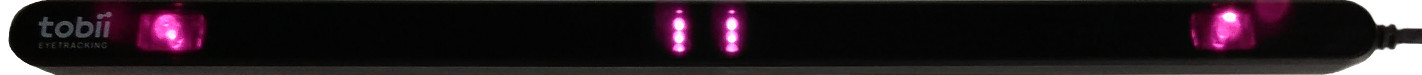
\includegraphics[width=0.95\textwidth]{eye_tracker.jpg}
    \caption{Picture of the Tobii Eye Tracker 4C in operation.}
    \label{fig.eyetracker}
\end{figure}

In order for the eye tracker to being able to track the gaze of the subject it must be calibrated.
A user-friendly calibration tool is included in the Tobii software package.
For each person different calibration data must be stored.
For this reason the Tobii software supports multiple user profiles which can be switched on the fly.
Given that in an economic experiment a workstation is used by a subject only once it is suggested to use the \emph{Guest} profile to store the eye tracker calibration data.
Once the eye tracker is calibrated for a subject, everything is ready.

\section{Execute 3rd Party Applications in \texttt{ztree}}
\label{sec.external}
In a first step, it is useful to define a global variable \texttt{Path} in a \texttt{ztree} program that points to the location of the toolset.

In order to define a path
\begin{enumerate}
    \item click on the last table in \texttt{Background}
    \item choose the menu \texttt{Treatment} $\rightarrow$ \texttt{New Program...}
    \item define the path of the installation folder of the \texttt{GazeToMouse} toolset, i.e.~\texttt{<GazeToMouse path>} as \texttt{Path} variable\\
        (e.g.~\texttt{Path="C:\textbackslash\textbackslash Users\textbackslash\textbackslash Max Muster\textbackslash\textbackslash Documents\textbackslash\textbackslash My Experiment\textbackslash\textbackslash GazeToMouse\textbackslash\textbackslash";}). \\
        Note that two backslashes are required for each path delimiter because in ztree \texttt{\textbackslash} is used as escape character.
\end{enumerate}

When writing the different stages of a \texttt{ztree} program, calls to external applications can be made.
This can be achieved as follows:
\begin{enumerate}
    \item click on the position where you want to include the call to the external program
    \item choose the menu \texttt{Treatment} $\rightarrow$ \texttt{New External Program...}
    \item choose \texttt{Run on z-Leaf}
    \item add the call to the external program to the field \texttt{Command Line} \\
        (e.g~a call to the guest calibration tool: \texttt{<><Path|-1>TobiiGuestCalibrate.exe}\\
        Note that the \texttt{Path} variable is used to indicate the location of the program.
        Figure~\ref{fig.extcall} shows an example of calling the Tobii guest calibration tool.
\end{enumerate}
\begin{figure}[ht]
    \centering
    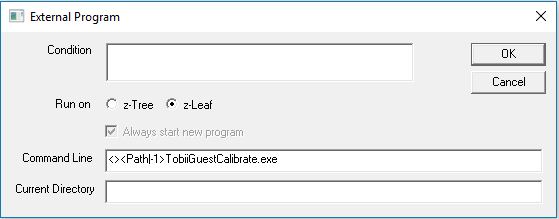
\includegraphics[width=0.6\textwidth]{ztree_extcall.png}
    \caption{External program call definition in \texttt{ztree}. The variable \texttt{Path} must be globally defined.}
    \label{fig.extcall}
\end{figure}

\chapter{Configuration of the \texttt{GazeToMouse} Toolset}
\label{sec.config}
The \texttt{GazeToMouse} toolset can be configured to work with different installations.
It allows to specify installation paths and gives some control over implemented features (e.g.~ mouse hiding or gaze filtering).
The Listing~\ref{lst.config} shows the default configuration values and provides a short explanation for each value.
\lstset{language=json}
\begin{lstlisting}[caption={Default configuartion values},label=lst.config]
{
    // the path to the output file
    "OutputPath": "",

    // the Tobii installation path
    "TobiiPath": "C:\\Program Files (x86)\\Tobii",

    // Path to the standard mouse pointer icon. This is used to restore the
    // mouse pointer. It has no effect if "HideMouse" is set to false
    "StandardMouseIconPath": "C:\\Windows\\Cursors\\aero_arrow.cur",

    // Tobii EyeX command to run a calibration
    "TobiiCalibrate": "Tobii EyeX Config\\Tobii.EyeX.Configuration.exe",

    // Tobii EyeX parameter to run a calibration
    "TobiiCalibrateArguments": "--calibrate",

    // Tobii EyeX command to run a guest calibration
    "TobiiGuestCalibrate": "Tobii EyeX Config\\Tobii.EyeX.Configuration.exe",

    // Tobii EyeX parameter to run a guest calibration
    "TobiiGuestCalibrateArguments": "--guest-calibration",

    // Tobii EyeX command to run calibration test
    "TobiiTest": "Tobii EyeX Interaction\\Tobii.EyeX.Interaction.TestEyeTracking.exe",

    // filter settings for the eye tracker
    //   0: unfiltered
    //   1: lightly filtered
    "GazeFilter": 0,

    // if set to true the mouse curser will be hidden by GazeToMouse.exe and
    // shown by GazeToMouseClose.exe
    "HideMouse": false
}
\end{lstlisting}
Note that the configuration file follows the \texttt{json} syntax which must not be violated.
If the following points are respected, no problem should arise:
\begin{itemize}
    \item the configuration values are enclosed in `\texttt{\{}' and `\texttt{\}}'.
    \item each configuration line ends with a `\texttt{,}'.
    \item the Windows path delimiter `\texttt{\textbackslash}' must be escaped (i.e.~ write `\texttt{\textbackslash\textbackslash}' when describing a path)
    \item \texttt{json} supports standard data types (e.g. integer, boolean, string).
        Use the same type as the default value.
    \item everything following a `\texttt{//}' is considered a comment.
\end{itemize}

Each executable of the toolset uses the same common configuration file.
The configuration file must be named \texttt{config.json} and is read from the following places with the indicated priority:
\begin{enumerate}
    \item in the directory of the caller, i.e~in \texttt{<zleaf path>}
    \item in the directory of the executables, i.e.~in \texttt{<GazeToMouse path>}
\end{enumerate}
If no configuration file can be found, the default values are used.

{\fontencoding{U}\fontfamily{futs}\selectfont\char 66\relax}
A word of warning when using the mouse hiding feature:
This feature hides the mouse when running \texttt{GazeToMouse.exe}.
If \texttt{GazeToMouse.exe} is forcefully closed or crashes the mouse pointer stays hidden.
For such cases the \texttt{ShowMouse.exe} utility can be used.

\section{Output File}
When running the program \texttt{gazeToMouse.exe} an output file is generated which holds the gaze coordinates of the user.
The output file is saved in the directory specified by \texttt{OutputPath} in \texttt{config.json}.
The name of the output file follows the form \texttt{<yyyyMMddTHHmmss>\_<hostName>\_gaze.txt} where

\begin{itemize}
    \item \texttt{<yyyyMMddTHHmmss>} is replaced by the timestamp indicating when the file was created (e.g. 20180129085521 stands for 2018.01.12 08:55:21).
    \item \texttt{<hostName>} is replaced by the name of the machine
\end{itemize}


\section{Log File}
All executables write continuously to the same log file.
This allows to track the eye tracker events that happened throughout a \texttt{ztree} session within one log file.
The log file is produced at the root directory of the application which is making the calls to the executables (e.g. at the location of zleaf.exe: \texttt{<zleaf path>}).

\end{document}
